\chapterimage{./Pictures/cover-stack}
\chapter{TP2 : Les Listes}
\textit{L'objectif de ce TP est de découvrir les listes avec l'utilisation de la classe \mintinline{java}{ArrayList}. On créera comme au TP1 des classes, ce qui nous permettra d'être encore plus à l'aise avec la programmation objet en JAVA}

\section{Exercice 1 : Classe Cours et tri de liste}
\textit{L'objectif de cet exercice est de créer une classe Cours. Cette classes possèdera comme attributs, un code, un intitulé et un volume horraire. Nous implémeterons un constructeur et nous surchargerons la méthode toString.}
\inputminted[linenos,firstline=3,lastline=63]{java}{../sources/src/tp2/Cours.java}

On ajoutera la méthode \mintinline{java}{verifyCode(String code)} afin d'enlever les caractère non alpha-numérique mis par l'utilisateur lors de l'instanciation de la classe ou encore lors de la mutation de l'attibut Code.
\inputminted[linenos,firstline=65,lastline=68]{java}{../sources/src/tp2/Cours.java}

\section{Exercice 2 : Classe Formation}
\textit{L'objectif de cet exercice est de créer une classe Formation, permettant de regrouper plusieurs cours. Cette classes possèdera comme attributs, un code, un intitulé et une liste de cours. Nous implémeterons un constructeur et nous surchargerons la méthode toString.}
\inputminted[linenos,firstline=5,lastline=66]{java}{../sources/src/tp2/Formation.java}

\section{Exercice 3 : Classe Main}
\textit{L'objectif de cet exercice est de simuler le scénario proposé en utilisant les classes créés précédemment. Pour cela, nous devrons comprendre et utiliser les méthodes fournies par la classe ArrayList.}
\\\\
Je crée la classe Main suivante :
\inputminted[linenos,firstline=3,lastline=46]{java}{../sources/src/tp2/Main.java}

À l'éxécution on obtient l'affichage suivant :
\begin{figure}[H]
  \centering
  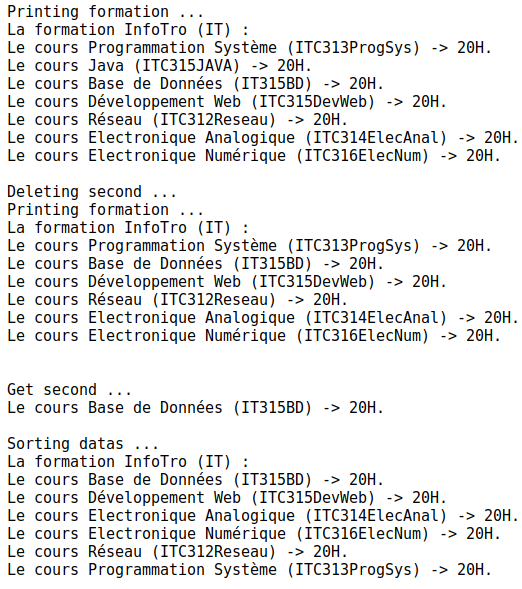
\includegraphics[width=300pt]{./tp/Pictures/tp2-execute}
  \caption{Exécution TP2}
  \label{Exécution TP2}
\end{figure}

\section{Exercice 4 : Trie de liste}
\textit{L'objectif de cet exercice est d'apprendre à implémenter les comportement d'une interface simple permettant de comparer les instances d'une classe et ainsi trier plus facilement les instances dans une collection par exemple.}
\\\\
Afin de pouvoir trier les objects d'un tableau nous devons surcharger la méthode \mintinline{java}{compareTo(Object o)} de l'interface \mintinline{java}{Comparable}.\\
Une interface permet à une classe d'implémenter un compartement réutilisable. Pour celà il faut utiliser le mot clef \mintinline{java}{implements} suivit de l'interface souhaiter pour implementer les méthodes de l'interface, ainsi pour l'interface \mintinline{java}{Comparable} servant à comparer les instances de la classe Cours nous feront comme ci-dessous :
\inputminted[linenos,firstline=3,lastline=3]{java}{../sources/src/tp2/Cours.java}

Ainsi nous pourront surcharger les méthodes de l'interface, ici la méthode \mintinline{java}{CompareTo(Object o)} qui comparera un maximum d'attributs de la classe comme ci-dessous :
\inputminted[linenos,firstline=52,lastline=63]{java}{../sources/src/tp2/Cours.java}

On utilisera de préférence la méthode \mintinline{java}{sort()} de l'instance plutôt que celle de la classe mère Collection, celà évitera les érreurs de type de Collection.\\
Nous pouvons si nous le voulons créer un comparateur à la voler en passant en paramètre \mintinline{java}{new Comparator(){}}, mais nous n'en avons pas l'utiliter ici.
\inputminted[linenos,firstline=41,lastline=41]{java}{../sources/src/tp2/Main.java}

\section{Synthèse personnelle}
Il existe plusieurs type de collection, facilitant toutes des manipulations précise.
\begin{itemize}
  \item ArrayList : permet à une collection d'assurer le stockage de donnés potentiellement dupliqués.
  \item HashSet : permet à une collection d'assurer l'unicité des donnés quelle contient.
  \item HashMap : permet de faire un dictionnaire.
  \item LinkedHashMap : permet de faire un dictionnaire ordonné.
  \item TreeMap : permet de faire un dictionnaire trié.
\end{itemize}

\begin{figure}[H]
  \centering
  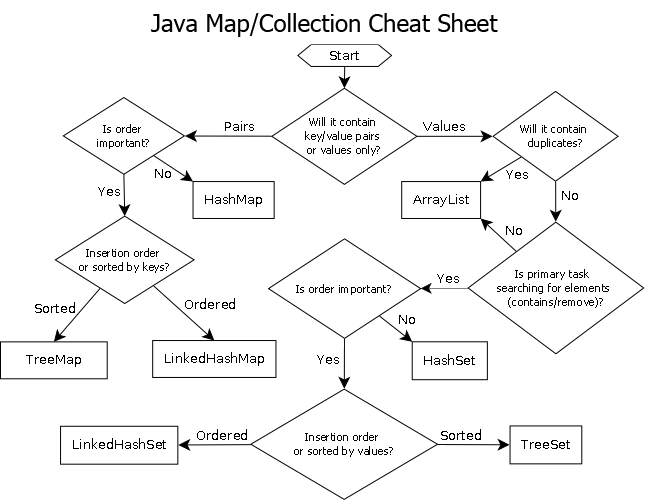
\includegraphics[width=400pt]{./tp/Pictures/tp2-collection-cheatsheet}
  \caption{Collection Cheatsheet}
  \label{Collection Cheatsheet}
\end{figure}

Comme nous avons pu le voir les Collections ont plusieurs avantages sur les tableaux. Nous en listons ci-dessous une liste exhaustive :
\begin{itemize}
  \item Muable
  \item Une API exhaustive contrairement aux tableaux.
  \item Peut être utilisé sur plusieurs threads sans danger.
  \item Accepte ou interdire les éléments null.
  \item Peut avoir des vues (unmodifiable, subList, filter...)
  \item Les méthodes \mintinline{java}{equals}, \mintinline{java}{hashCode} et \mintinline{java}{toString} d'une collection réponse aux attentes d'un utilisateur, ces même méthodes sur un tableaux sont souvent sujet à des bugs.
\end{itemize}
